\section{Methods}
\label{sec:methods}

\subsection{Method Overview}
This pipeline implements a fully automated, iterative 3D Gaussian Splatting (3DGS) reconstruction system using a Actor-Critic agent architecture built on LangGraph. The system transforms raw video input into a refined 3D scene through a feedback loop between an Actor and Critic agent, removing the need for manual hyperparameter tuning that traditionally is in 3DGS workflows.

\subsection{System Architecture}
We create 3D scene reconstructions through a collaborative system of prefiltering, followed by a refinement loop with the Actor and Critic agents. Our most important contribution is the autonomous, iterative approach to 3DGS using the Actor-Critic architecture. 

\begin{figure*}[h]
    \centering
    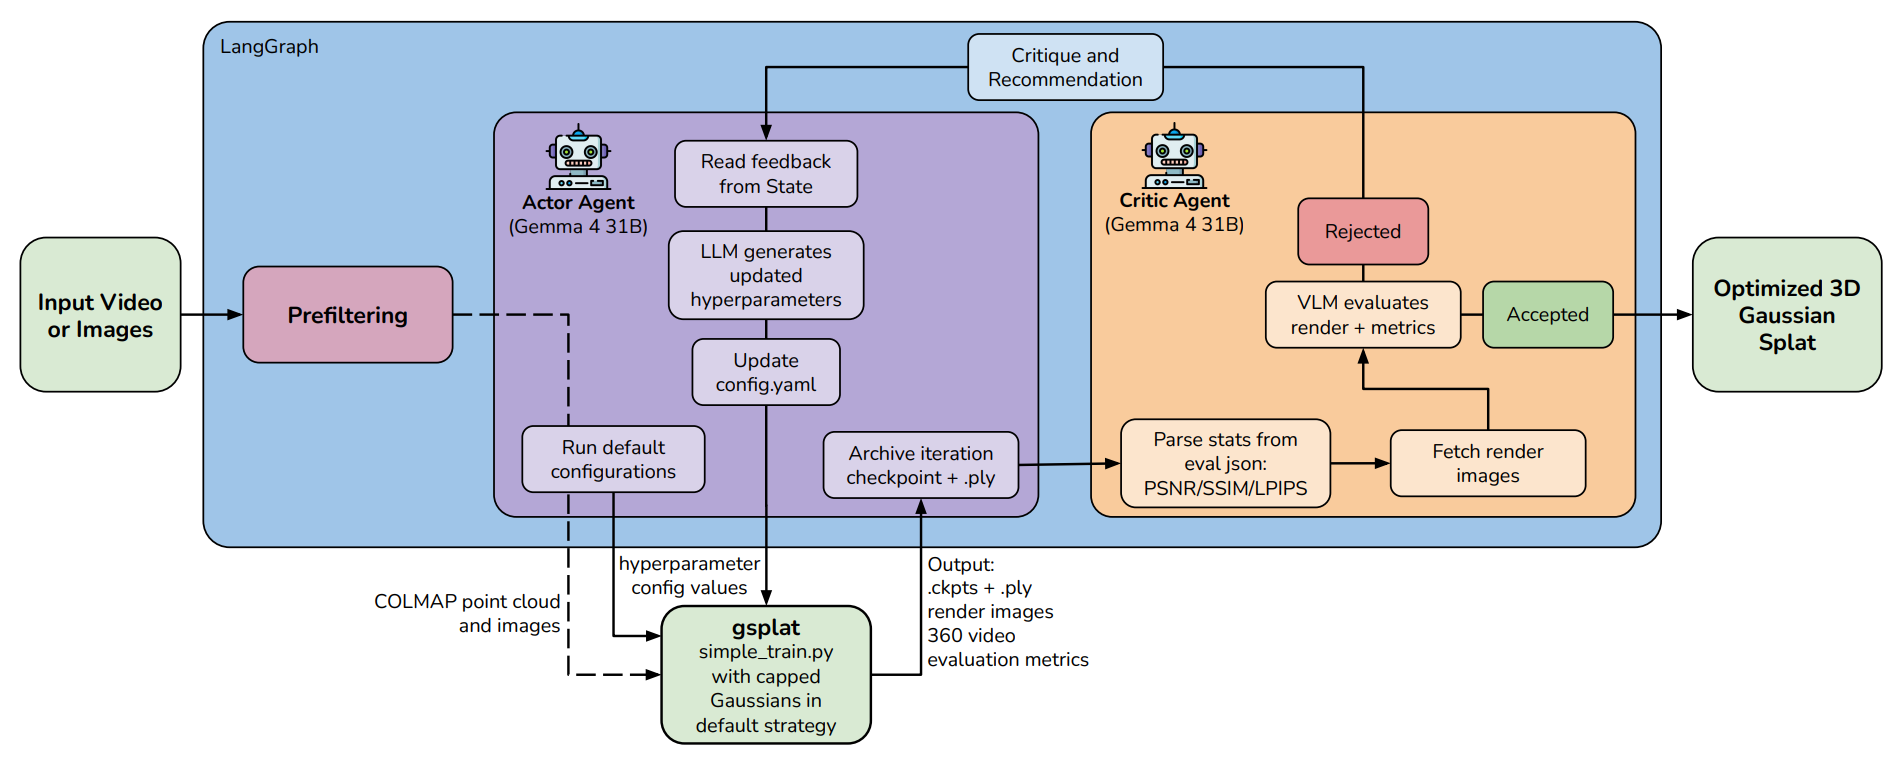
\includegraphics[width=\linewidth]{images/pipeline_diagram.png}
    \caption{Agentic Workflow Diagram}
    \label{fig:agentic_diagram}
\end{figure*}

\subsection{Method Details}
\subsubsection{Agent Roles}
\noindent The Actor Agent's job is to mutate the configuration state of the Gaussian Splatting reconstruction. The actor holds the current config file containing parameters such as number of Gaussians, densification interval, learning rates for position/opacity/scale/rotation, spherical harmonics degree, pruning thresholds, and camera pose refinement flags and applies edits to it based on structured feedback it receives from the Critic. Instead of doing generation from scratch for each iteration, the Actor applies edits such as "increase the densification interval from 100 to 150 steps. The Actor receives the Critic's structured feedback, reasons about which config parameters are causally responsible for the reported artifact, proposes a change to the config, applies it, triggers a re-train or re-optimize pass via gsplat, and then passes the newly rendered output back to the Critic for the next round. This gradient-free optimization loop over the config space, driven by visual and geometric feedback, is better than a loss function, because many failure modes in 3DGS (e.g. floaters, needle Gaussians, blurry textures, background collapse) are not easily encoded as a differentiable objective function.\\

\newpage
\noindent\title{Actor Agent Prompt:}
\begin{figure}[h]
\centering
\begin{verbatim}
prompt = (
    "You are an expert ML Engineer 
    specializing in 3D 
    Gaussian Splatting.\n"
    "A visual critic has reviewed the 
    latest render and provided 
    this feedback:\n\n"
    f"{state['feedback']}\n\n"
    "Current training config:\n"
    f"{current_config_str}\n"
    "Return updated hyperparameters in 
    .json format to address 
    the critique.\n"
    "Do not increase max_steps past 
    50,000, and only increase it 
    in smaller increments 
    if necessary.\n"
    "Do not increase max_num_gaussians
    past 1,000,000, and only increase 
    it in smaller increments 
    if necessary.\n"
    )
\end{verbatim}
\caption{Example Actor Agent Prompt}
\label{fig:actor-agent-prompt}
\end{figure}

\noindent The Critic Agent's job is to look at the rendered 3DGS output and produce structured, actionable feedback that the Actor can use to change specific parameters. The Critic will inspect the scene from multiple angles. It examines close-up views of problematic regions, depth maps to detect geometric inconsistencies, opacity visualizations to catch floaters, and normal maps to identify surface reconstruction failures\\

\noindent For the Critic agent, we used Google Gemma 4 31B IT as the VLM. We take inspiration from frameworks like Feature4X, where gpt-4o act as high-level agents for executing and refining complex scene manipulations. In our architecture, the VLM Critic functions as an expert diagnostic layer. By analyzing a multi-view grid of renders alongside depth and opacity buffers, the agent can pinpoint specific optimization failures. For instance, the Critic might identify that “inward-pointing needle Gaussians on a ceiling” suggest a lack of upward-facing or overhead views. Alternatively, it could recognize that a “foggy” floor surface indicates an insufficient spherical harmonics degree, preventing the model from resolving sharp, view-dependent reflections.\\

\noindent\text{Critic Agent Prompt:}
\begin{figure}[h]
\centering
\begin{verbatim}
prompt = (
    "You are an expert Machine 
    Learning Critic specializing 
    in 3D Gaussian Splatting.\n"
    "Analyze the rendered 
    novel viewpoints 
    above alongside these 
    training metrics:\n\n"
    f"{metrics_str}\n\n"
    "Look specifically for:\n"
    "1. Floaters / clouding (foggy 
    artifacts in empty space)\n"
    "2. Blurring (loss of 
    fine surface detail)\n"
    "3. Anisotropic stretching 
    (needle-shaped Gaussians)\n\n"
    "Reply in exactly this format:\n"
    "STATUS: ACCEPTED or REJECTED\n"
    "CRITIQUE: <one sentence 
    assessment>\n"
    "RECOMMENDATION: <specific 
    hyperparameter adjustments 
    if REJECTED, else None>"
    )
\end{verbatim}
\caption{Example Critic Agent Prompt}
\label{fig:critic-agent-prompt}
\end{figure}


\noindent The design constraint is that the Critic's output must be structured enough for the Actor to parse and act on a typed schema rather than a free-text paragraph the Actor has to interpret. This structured output lets us replay the full sequence of Critic observations and Actor edits to understand exactly how the scene evolved across iterations.

\noindent\text{Critic Agent Feedback:}
\begin{figure}[h]
\centering
\begin{verbatim}
"STATUS: ACCEPTED or REJECTED\n"
"CRITIQUE: <one sentence assessment>\n"
"RECOMMENDATION: <specific 
hyperparameter adjustments 
if REJECTED, else None>"
\end{verbatim}
\caption{Example Critic Agent Feedback}
\label{fig:ex-critic-agent-feedback}
\end{figure}

\subsubsection{Representations}
The Prefiltering tool passes the COLMAP processed point clouds of the input frames into the Actor/Critic cycle. As the Actor and Critic work together through iterations, the Actor changes parameters within the Gaussian Splatting training configuration in .yaml format.

\noindent\text{Sample Config.yaml:}
\begin{figure}[h]
\centering
\begin{verbatim}
{
 training:
    densify_grad_threshold: 0.0002
    densify_size_threshold: 0.05
    max_num_gaussians: 500000
    max_steps: 2000
    opacity_cull_threshold: 0.005
}
\end{verbatim}
\caption{Example Training Config}
\label{fig:json-schema}
\end{figure}

\noindent After completing the GS training, the Actor agent passes a select number (4) of rasterized views of the GS to the Critic. The Critic agent will represent feedback in a structured prompt format, such that the Actor agent can easily interpret it and determine how to iterate based on the feedback.

\subsection{Implementation}

\subsubsection{Overview}
\noindent The pipeline is implemented in Python 3.10 using LangGraph infrastructure to build our iterative workflow. The LangGraph state contains directory paths, file names, feedback from the critic agent, current iteration, and path for the point cloud generated by pycolmap. Both agents use "gemma-4-31b-it" as the default, and fall back on to "gemma-4-26b-a4b-it" if there is a Google server API error.\\

\noindent The prefiltering process first uses Python ffmpeg with GPU acceleration to downsample and select frames. The selected frames are then passed to COLMAP, a Structure from Motion (SfM) technique, to create the point cloud for initializing the Gaussian Splatting process. COLMAP outputs several files, including images.bin, cameras.bin, and points3d.bin, which are essential files for training the Gaussian splatting. We used pycolmap with GPU acceleration to create the COLMAP outputs. The pre-filtering process can also be skipped if the user already has a COLMAP output by adding the –skip\_prefiltering flag when running the agents.\\

\noindent The Actor agent starts with initial configuration values for the first agentic loop, which are passed into gsplat’s simple\_trainer.py to train the 3DGS reconstruction. The gsplat function also takes in the directory storing the COLMAP outputs and the output directory location. At the first agentic loop the actor agent is fed with a set of default hyperparameters After the first agentic loop, the LLM is asked to update the hyperparameters given an initial prompt, the feedback from the Critic agent, and the current configuration values. The response is then parsed and written to config.yaml before gsplat is trained again using the new parameters.\\

\noindent The Critic agent evaluates the reconstruction based on several components, including the following metrics: PSNR, SSIM, and LPIPS. The Critic agent is sent four rendered frames which are rasterized novel view images of the 3D reconstruction. These frames are from different viewpoints of the 3D reconstruction. The VLM is provided the metrics and image, and is prompted to provide a structured response for the following with an emphasis on floaters, blurring, and needle-shaped Gaussians: whether the reconstruction is accepted or rejected, critiques, and recommended hyperparameter changes. The structured response is in the form of a class that contains the hyperparameters that the Critic agent modifies. These hyperparameters are max\_steps, opacity\_cull\_threshold, densify\_grad\_threshold, densify\_until\_step, densify\_size\_threshold, and max\_num\_gaussians. If the VLM accepts the reconstruction, the loop ends; otherwise, the response is passed to the Actor agent to update the training configuration in order to further refine the scene.

\subsubsection{Implementation Details}
\noindent In order to limit our agent-critic pipeline to similar runtime and memory budget for each agentic loop, we modified gsplat’s default densification strategy (the original 3DGS adaptive density control) to include a cap\_max parameter for loosely capping the number of Gaussians, based on the MCMC implementation for max\_num\_gaussians. Each iteration of the Gaussian splatting optimization includes a densification and a pruning phase – when the number of Gaussians surpasses cap\_max to a certain degree, the densification phase of the next phase is skipped so that Gaussians are pruned further first. Although gsplat also supports the MCMC densification strategy, which has a fixed cap on the number of Gaussians built in, we hypothesize that the other parameters supported by MCMC are not well-suited to our needs. For example, noise\_injection\_stop\_iter is the iteration at which the MCMC strategy stops injecting noise into Gaussian positions, and would not be a parameter that the critic agent and actor agent are well-equipped to modify, because it is not immediately observable from the rasterized outputs. We conducted experiments with both of these densification strategies, which we discuss further in the Results section.\\

\noindent Although the Google AI Studio SDK supports structured output that matches a typed object (for our purposes, the Gaussian splatting configuration parameters), we still observed non-parseable outputs that required some more post-processing.


\subsubsection{Evaluation Details}
\noindent In order to test our pipeline, we utilized a sample video in 4K resolution from the DL3DV-10K dataset. To ensure reconstruction quality, we use PSNR, SSIM, and LPIPS as they measure image quality from three distinct perspectives: signal, structure, and perception. We assess absolute pixel fidelity using PSNR, structural and edge consistency via SSIM, and high-level feature realism through the deep perceptual metric LPIPS.